\chapter{Design of a Mitosis Detection algorithm}
\label{chapter4}
\thispagestyle{empty}

\begin{quotation}
{\footnotesize
\noindent \emph{``Ab uno\\ disces omnis''}\\
\noindent (Learn everything from one)
\begin{flushright}
Publius Vergilius Maro (Aeneis II, 65-66)
\end{flushright}
}
\end{quotation}

\vspace{0.5cm}

%\noindent In questa sezione si spiega come \`e stato affrontato il problema concettualmente, la soluzione logica che ne \`e seguita senza la documentazione.

We developed an algorithm to perform mitosis-detection as a part of our work, with the aim to compare its results with humans facing the same task.

\section{Dataset}

We used the public MITOS dataset \cite{icpr}. The dataset is composed by a total of 50 2084$\times$2084 pixel images
covering an area of 512$\times$512 $\mu$m each, acquired with an APERIO XT scanner (see Figure \ref{ch2:fig1}). 
A unique split is defined by the dataset authors, with 35 images used for training and 15 for evaluation.
The dataset contains a total of about 300 mitosis, which were annotated by an expert pathologist.
The performance of the algorithms participating to the \textit{2012 ICPR mitosis detection contest} are shown in Section \ref{ch3:icpr_perf}.\\
With reference to Figure \ref{ch3:fig1}, we focused on on the classification subproblem, with the \Glspl{ROI} given as an input.
The input is given in form of an image patch with size 100$\times$100 pixel: such size completely contains the image of the cell.
The task is to map each patch to one of two classes:
\begin{itemize}
 \item [] \textit{\textbf{C1}}: the image contains a mitosis at its center,
 \item [] \textit{\textbf{C0}}: the image does not contain a mitosis anywhere. 
\end{itemize}

There are no samples in which a mitosis is visible off-center.

\vspace{0.5cm}

\subsection{Image Candidates}

For the \textit{\textbf{C1}} class, all the 216 mitosis available in the 35 training images are chosen
as training samples, and all 87 mitosis in the evaluation images are chosen as
evaluation samples.\\
We enforced an even distribution of the two classes classes both in training and in evaluation sets, and therefore
selected 216 \textit{\textbf{C0}} samples for training, and 87 \textit{\textbf{C0}} samples for evaluation; the resulting
training set contained 432 samples.\\
Millions of different \textit{\textbf{C0}} samples may be randomly chosen from the original training and evaluation images:
an overwhelming majority of such samples would not contain any nucleus and be non-informative for training and trivial for
evaluation. Limiting the choice to non-mitotic nuclei \texttwelveudash{} which greatly outnumber
mitotic ones \texttwelveudash{} would not solve the problem, since most of such nuclei look very
similar to each other and are trivially identified as non-mitotic. Only a small
subset of non-mitotic nuclei \texttwelveudash{} as well as other structures and artifacts \texttwelveudash{} pose an
actual challenge, both for humans and for algorithms.\\
In order to select such objects as \textit{\textbf{C0}} samples, we used the output produced by a simple \Gls{CNN}-based mitosis detector,
similar to the one outlined in \cite{agNN} for selecting useful training samples.
The detector, built at IDSIA, was trained on few images in the training set, then applied on the whole dataset.
Because the detector was simple and trained on a small amount of data, it performed poorly and detected a lot of false positives.
\textit{\textbf{C0}} samples have been randomly chosen among the outputs of such detector which are
farther than 50 pixels from the centroid of any mitosis; this ensures that no actual
mitosis is visible in the corresponding image patch. The resulting samples do in
fact resemble mitosis, are informative in the training set, and appear non-trivial
in the evaluation set. Finally, 10 \textit{\textbf{C0}} samples in the evaluation set are substituted
with 5 random false positives obtained from each of the two best performing
algorithms (IDSIA and IPAL). These last 10 samples are particularly useful to compare humans to algorithms, in fact allowed us to better observe how test subjects
behave on the algorithms’ false positives, which are rare in the evaluation set because
algorithms were tuned to solve a problem with very low prevalence of mitotic samples.


\vspace{0.5cm}

\subsection{Extended Dataset}

We extended our dataset by rotating and mirroring each image patch (see Figure \ref{ch4:fig1}). We used the extended dataset only for the detection algorithm, so that we could analyze
the effect of different features, which can be explicitly dependent on orientation or not, on the global performance of the classifier.\\
In case of extended dataset, the classification of a single image patch becomes the average of the classifications obtained on the 8 samples.

\begin{equation}
 c_{i} = \frac{\sum_{j=1}^{8} c_{ij}}{8}
\end{equation}

Where $c_{i}$ represents the classification of image patch \textit{i}, and $c_{ij}$ represents the classification of variation \textit{j} of image patch \textit{i} .



\begin{figure}[!hbt]
  \centering
    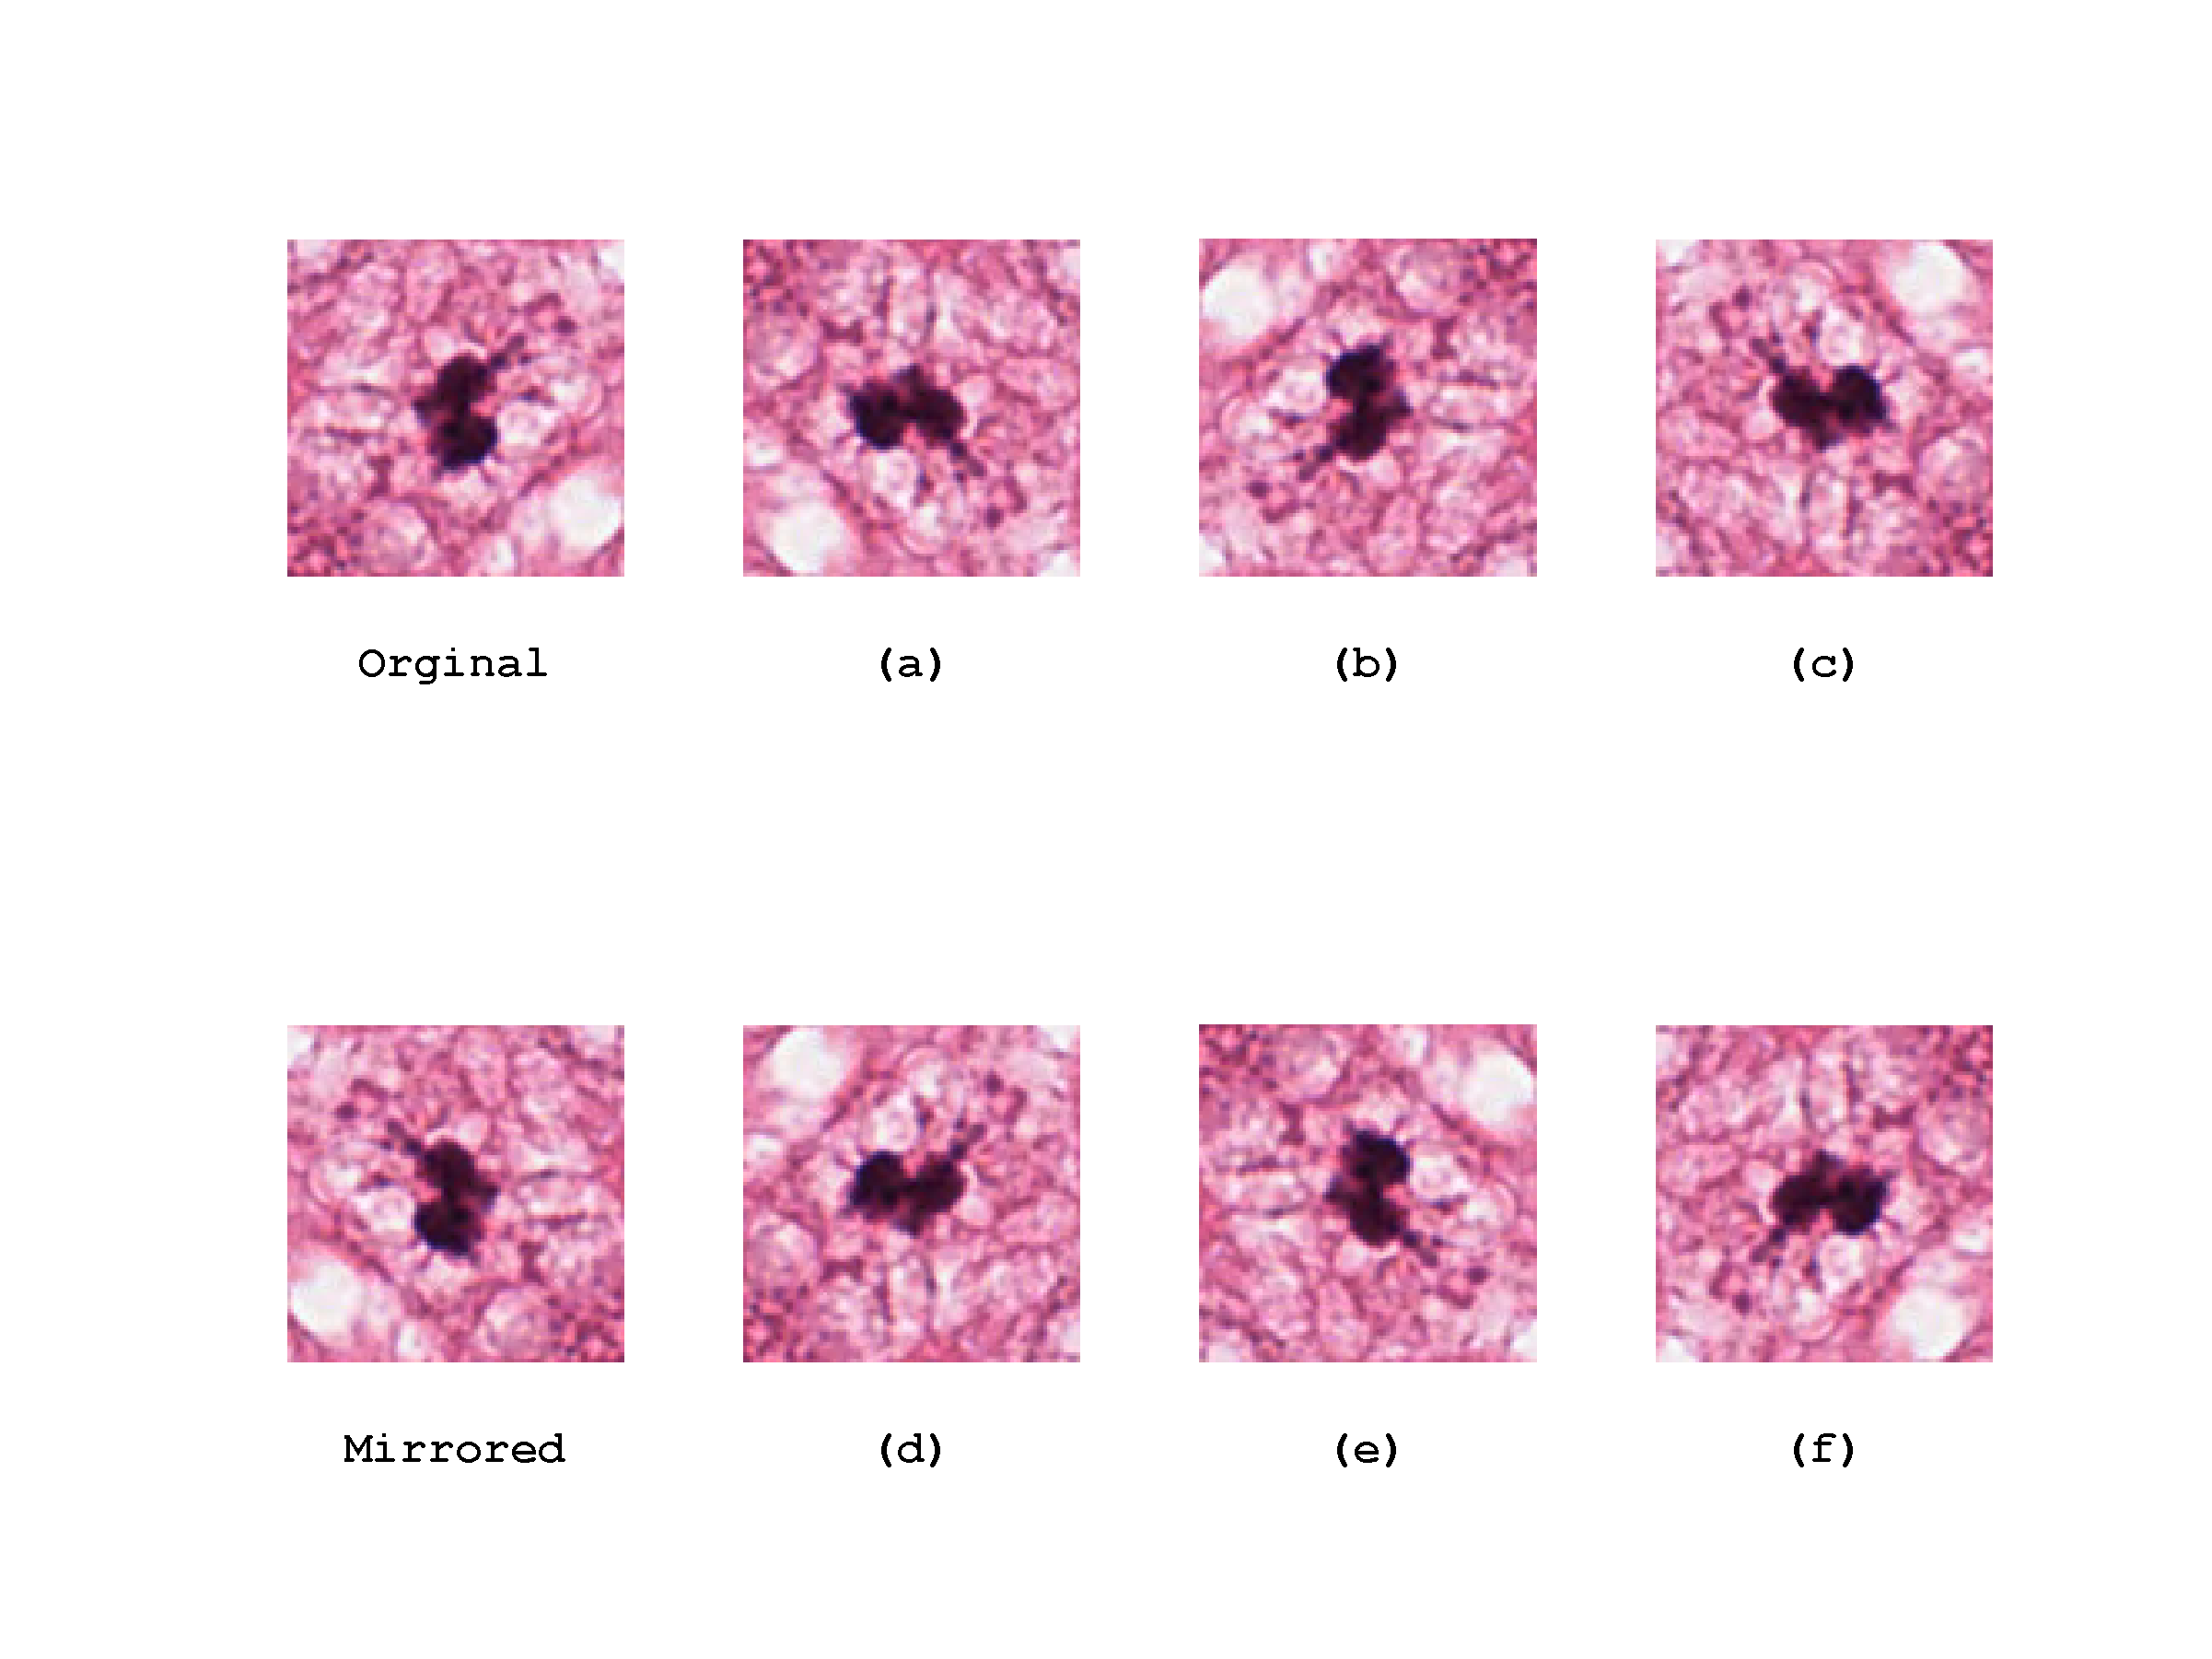
\includegraphics[width=0.94\textwidth]{./images/rotDataset.png}
  \caption[Extended Dataset]{Extended dataset\\(a),(b),(c): $\pi/2$ clockwise rotations, (d),(e),(f): mirror and $\pi/2$ clockwise rotations.}
  \label{ch4:fig1}
\end{figure}  

\vspace{0.5cm}




\section{Features Extraction}

Each image patch can be represented as a 100$\times$100$\times$3 matrix, where the $(i,j,:)$ triplet represents the RGB value of point with coordinates $(i,j)$ in the image.
Each value is in the range 0 to 255. Starting from these (raw) data we extracted some features by which we trained and tested our classifiers.

\vspace{0.5cm}

\subsection{Simple Features}

The simplest features that can be computed involve the average and the standard deviation of the RGB values of the image patch. They can be computed on all the data or can be maintained separated
for each RGB component. In the first case, average and standard deviation each give one value every instance:

\begin{eqnarray}
 m & = & \frac{1}{100\times100\times3} \left( \sum_{i=1}^{100} \sum_{j=1}^{100} \sum_{k=1}^{3} i_{ijk} \right) \\
 \sigma & = & \sqrt{\frac{1}{100\times100\times3} \left( \sum_{i=1}^{100} \sum_{j=1}^{100} \sum_{k=1}^{3} (i_{ijk} - m )^2 \right)}
\end{eqnarray}

Otherwise, average and standard deviation produce a vector of three components:

\begin{eqnarray}
 \overline{M} & = & \left[ \begin{array}{c}
                            \frac{1}{100\times100} \left( \sum_{i=1}^{100} \sum_{j=1}^{100} i_{ij1} \right) \\
                            \frac{1}{100\times100} \left( \sum_{i=1}^{100} \sum_{j=1}^{100} i_{ij2} \right) \\
                            \frac{1}{100\times100} \left( \sum_{i=1}^{100} \sum_{j=1}^{100} i_{ij3} \right)
                           \end{array} \right] \\
 \overline{\sigma} & = & \left[ \begin{array}{c}
                                 \sqrt{\frac{1}{100\times100} \left( \sum_{i=1}^{100} \sum_{j=1}^{100} (i_{ij1} - M(1) )^2 \right)} \\
                                 \sqrt{\frac{1}{100\times100} \left( \sum_{i=1}^{100} \sum_{j=1}^{100} (i_{ij2} - M(2) )^2 \right)} \\
                                 \sqrt{\frac{1}{100\times100} \left( \sum_{i=1}^{100} \sum_{j=1}^{100} (i_{ij3} - M(3) )^2 \right)}
                                \end{array}  \right]
\end{eqnarray}

Another simple set of features is represented by the \textit{median} of each RGB values. 

%	-	m: mean
%	-	s: standard deviation
%	-	i: mean intensity in 25 central regions of the image
%	-	M: mean per color
%	-	S: std per color
%	-	d: median per color



\vspace{0.5cm}

\subsection{Color Histograms}

%	-	H: color histograms (16 bins)



\vspace{0.5cm}

\subsection{Texture Features}

%	-	l: lbp riu2 radius 1, 8 neighbors
%	-	v: mean pixel variance
%	-	L: lbp riu2 radius 1-2-3, 8 neighbors concatenated
%	-	r: lbp ri radius 1, 8 neighbors
%	-	u: lbp u2 radius 1, 8 neighbors
%	-	V: pixel variance, 36 elements
%	-	R: lbp ri radii 1-2-3, 8 neighbors
%	-	U: lbp u2 radii 1-2-3, 8 neighbors



\vspace{0.5cm}


\section{Classifiers}

In our work we focused on two types of classifiers: \textit{Support Vector Machines} and \textit{Random Forests}
which are widely used in computer vision classification problems ( e.g. \cite{mitosisDetectionLearningBased} and \cite{randForests04}).
We also mention \Glspl{CNN} because they played a relevant role in the definition of our dataset [REF].


\vspace{0.5cm}

\subsection{Support Vector Machines}




\vspace{0.5cm}

\subsection{Random Forests}




\vspace{0.5cm}


\section{Experiments}



\vspace{0.5cm}

\subsection{Exp.1: }


\vspace{0.5cm}

\subsection{Exp.2: }


\vspace{0.5cm}

\subsection{Exp.3: }


\vspace{0.5cm}

\subsection{Exp.4: }


\vspace{0.5cm}

\subsection{Exp.5: }


\vspace{0.5cm}

\subsection{Exp.6: }

Curse of dimensionality and PCA

[SNIPPET]
In most computer vision applications it is not sufficient to extract only one type of feature to obtain the relevant information from the image data.
Instead two or more different features are extracted, resulting in two or more feature descriptors at each image point.
A common practice is to organize the information provided by all these descriptors as the elements of one single vector,
commonly referred to as a feature vector. The set of all possible feature vectors constitutes a feature space.
A common example of feature vectors appears when each image point is to be classified as belonging to a specific class.
Assuming that each image point has a corresponding feature vector based on a suitable set of features,
meaning that each class is well separated in the corresponding feature space, the classification of each image point can be done using standard classification method.



\vspace{0.5cm}

\subsection{Exp.7: }


\vspace{0.5cm}





 


